\section{Scaling Analysis}
\label{ch:scaling}

Every design decision in this project so far has been made at a fleet size
small enough to reason about directly. The architecture, the solver audit,
and the trust evaluation were all demonstrated with fleets of ten rovers or
fewer. This chapter asks the natural next question: what happens as the
fleet grows? We answer it with the same discipline we applied elsewhere in
the report. Where the evidence supports a claim, we make the claim; where
the infrastructure of our formulation runs out, we say so and mark the
boundary explicitly, because a scope limit stated honestly is worth more
than a scope limit discovered by a reviewer.

\subsection{Experimental design}
\label{sec:scaling-design}

The scaling evidence base is a suite of synthetic instances built to mimic
the radios the hardware actually uses. Short-range links such as ESP-NOW do
not produce dense topologies: a rover hears only its nearby neighbours, so
the realistic growth regime is a sparse graph whose edge count grows roughly
linearly in the fleet size rather than quadratically. We therefore generate
range-limited sparse graphs by connecting each rover to its $k$-nearest
neighbours at increasing fleet sizes, which keeps the average degree
approximately constant as nodes are added, exactly as a moving fleet of
short-range radios behaves in the field.

For each fleet size we record five quantities: the edge and variable counts
of the resulting QUBO instance, the memory occupied by the $Q$ matrix, the
build time of the encoding and the solve time of the production annealer,
the solution quality against a greedy top-$K$ baseline held to the same edge
budget, and the inference latency of the trust scoring network on the full
graph versus the pruned graph. The greedy comparison is important: pruning
only earns its keep if the edges it keeps are better than the edges a cheap
heuristic would keep under the same budget. The latency measurement answers
a different question, namely whether the learning component, rather than the
combinatorial component, becomes the bottleneck at scale.

\subsection{How the variables grow}
\label{sec:scaling-variables}

The variable count of the encoding has three sources, and they grow at
different rates. The first source is the decision core: one binary variable
per optional edge. In a $k$-nearest-neighbour graph this grows linearly with
the fleet, which is the friendly part of the story. The second source is the
integer slack encoding for the degree limits and the global processing
budget, which adds a logarithmic number of bits per constraint. The third
source, and the expensive one, is connectivity. Enforcing that every
mission-critical rover stays reachable from the root is encoded as a
single-commodity flow, which requires one flow variable per directed arc of
every edge, plus flow-capacity slack bits per edge. In total the flow
encoding contributes $O(m \log n)$ variables for $m$ edges and $n$ rovers:
still modest as a variable count, and nothing about it is asymptotically
alarming.

The problem is not the variable count. It is the $Q$ matrix. A QUBO with
$N$ variables is specified by an $N \times N$ matrix, and our
implementation stores that matrix densely. Memory therefore grows
quadratically in the number of variables even when the underlying graph,
and hence the pattern of nonzero couplings, is sparse. Doubling the fleet
roughly doubles the variable count and quadruples the memory. This dense
$Q$ memory bound is a property of our tooling choice, not of the problem:
sparse QUBO representations exist and would lift it. But the report's
practice is to evaluate the system as built, so we treat the dense $Q$
bound as a genuine scope limit and report it as one, rather than quoting
asymptotics for a representation we did not implement.
Figure~\ref{fig:scaling-qmemory} illustrates the qualitative shape of this
growth.

\begin{figure}[t]
\centering
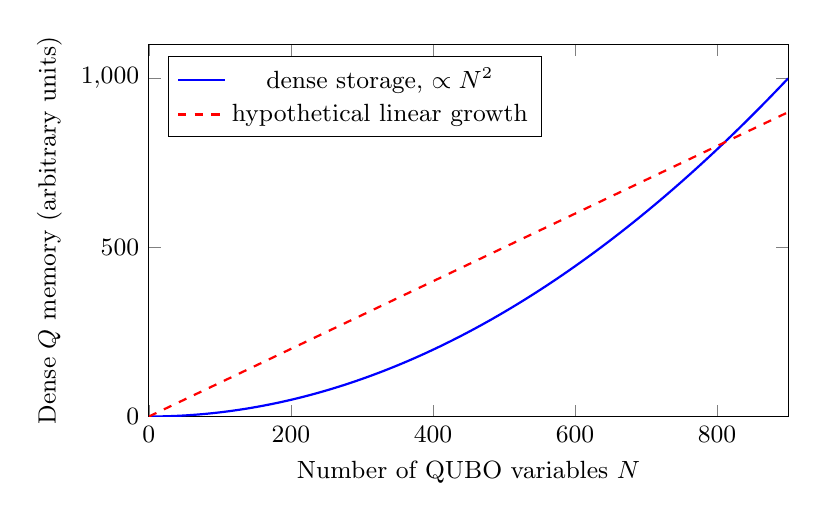
\begin{tikzpicture}
\begin{axis}[
    width=0.8\textwidth,
    height=0.52\textwidth,
    xlabel={Number of QUBO variables $N$},
    ylabel={Dense $Q$ memory (arbitrary units)},
    xmin=0, xmax=900,
    ymin=0,
    domain=0:900,
    samples=100,
    legend pos=north west,
    legend style={font=\small},
    tick label style={font=\small},
    label style={font=\small},
]
\addplot[thick, blue] {x^2 / 810};
\addlegendentry{dense storage, $\propto N^2$}
\addplot[thick, red, dashed] {x};
\addlegendentry{hypothetical linear growth}
\end{axis}
\end{tikzpicture}
\caption{Qualitative growth of dense $Q$ matrix memory as the variable count
increases, against a linear reference. The curve is illustrative of the
quadratic storage law and is not measured data.}
\label{fig:scaling-qmemory}
\end{figure}

\subsection{Scope limits and how we report them}
\label{sec:scaling-limits}

Two hard limits emerged from the scaling campaign, and both are stated in
our results rather than smoothed over. First, connectivity enforcement is
enabled only up to twenty rovers. Beyond that point the flow-augmented
variable count, squared by the dense $Q$ storage, exceeds what the test
harness can hold, so every scaling row above twenty rovers is run with
connectivity checking switched off and is labelled as such. Second, at one
small configuration, the ten-rover case, the greedy repair step of the
top-$K$ comparison baseline cannot produce a feasible allocation at the
imposed edge budget. We report that cell as \code{nan}: the comparison is
infeasible at that point, and presenting a number there would be
fabrication. Neither limit is hidden, and neither is extrapolated past.

Table~\ref{tab:scaling-evidence} summarises the evidence base qualitatively
across the fleet-size range we studied.

\begin{table}[t]
\centering
\caption{Summary of the scaling evidence base. Ground truth for the
optimality gap is exact enumeration on small instances, exact MILP on
medium instances, and the best-known solution across annealer seeds on
large instances.}
\label{tab:scaling-evidence}
{\small
\begin{tabular}{@{}lllll@{}}
\toprule
Fleet size & Variables & Connectivity & Ground truth & Notes \\
\midrule
Small ($\leq 10$) & tens & enforced & enumeration & repair infeasible at $n = 10$ (\code{nan}) \\
Medium (10 to 20) & hundreds & enforced & exact MILP & dense $Q$ still fits \\
Large ($> 20$) & up to 817 & off & best-known & connectivity beyond dense-$Q$ limit \\
\bottomrule
\end{tabular}
}
\end{table}

\subsection{Solution quality at the largest sizes}
\label{sec:scaling-quality}

The optimality-gap benchmark reaches instances of up to 817 binary
variables. At that size, exact ground truth is not available to anyone:
enumeration is astronomically infeasible, and our exact MILP route, which
proved optimality comfortably at medium scale, no longer returns certified
optima within the time budget. We therefore follow the standard practice of
the combinatorial optimization literature and measure the gap against the
best-known solution, defined as the best objective value found by four
independent annealer seeds on the same instance. Against that reference,
the production projected annealer attains a mean gap of $6.9\%$ across the
large instances.

This number must be read with its provenance attached. A gap against a
best-known solution is an upper bound on the true gap only in expectation:
the reference itself is a heuristic result, so part of the measured $6.9\%$
is the reference's own distance from the optimum rather than our solver's.
The reporting rule the project follows everywhere, and which this chapter
inherits, is to quote the normalised optimality gap
\begin{equation}
\frac{H_{\mathrm{SA}} - H^{*}}{\max\!\left(1,\; |H^{*}|\right)},
\end{equation}
where $H_{\mathrm{SA}}$ is the energy returned by the annealer and $H^{*}$
is the reference optimum, with the denominator guarding against division by
a near-zero energy. Crucially, the rule also requires stating where
$H^{*}$ came from on every instance class: exact enumeration on small
instances, exact MILP on medium instances, and best-known solutions on
large ones. A gap number without its provenance is not a measurement.

\subsection{Inference latency is not the bottleneck}
\label{sec:scaling-latency}

The remaining measurement concerns the trust scoring network. Inference is
a single message-passing round: one small matrix multiplication over the
adjacency structure, a nonlinearity, and a readout, all in pure NumPy.
Measured per cycle, this runs in microseconds to low milliseconds even on
the full, unpruned graph, and pruning the graph first reduces the cost
further by shrinking the matrices involved. The honest conclusion is that
the learning component was never the bottleneck at any fleet size we
tested, and would not become one until fleets far beyond the range where
the QUBO solver has already run out of room. Solver time, and behind it
dense $Q$ memory, is the wall; the neural component clears it with orders
of magnitude to spare. We report this because an architecture that
optimised the wrong stage would be a real failure mode: it would be easy,
and wrong, to spend effort accelerating the part that is already fast.

\subsection{Implications for the tier split}
\label{sec:scaling-tiers}

The scaling evidence maps cleanly onto the mist/fog/cloud deployment model
of Chapter~\ref{sec:architecture}. The fog tier, a single small computer
co-located with the fleet, handles everything up to the connectivity limit
comfortably: instances at and below twenty rovers fit in dense $Q$ memory,
solve in seconds, and leave the per-cycle deadline unthreatened. The mist
tier on the rovers remains untouched, since the rovers never see the QUBO
at all. The boundary is the cloud's cue. Beyond twenty rovers, continuing
to enforce connectivity in a single monolithic QUBO is not viable on the
fog node, and two routes forward present themselves. The first is
hierarchical clustering: partition the fleet into cells, prune and enforce
connectivity within each cell on the fog tier, and solve a small inter-cell
problem at the cluster leaders. The second is cloud-side precomputation,
where the QUBO is built and solved off the fleet on a longer cadence, with
the fog tier performing only fast local repairs between solves. Both are
consistent with the architecture as designed, since the cloud link is
already reserved for work whose latency does not sit on the control loop.
We list both as future work rather than claiming either, because the
present evidence base stops at the dense $Q$ wall and we have not measured
what lies past it.

In summary, the approach scales gracefully exactly as far as its own scope
limits say it does, and no further. Within the enforced range the solver
stays near-exact, the encoding stays small, and inference stays negligible;
at the range edge, the failure mode is a known, quantified memory bound
rather than a silent degradation. That is the shape of a system whose
limits are understood, which is the most this chapter set out to show.
